\newcommand\legendas[1]{\begin{footnotesize}#1\end{footnotesize}}

\chapter[Introdução, por Ricardo Lísias]{introdução}
\hedramarkboth{ricardo lísias}{introdução}

Quando, depois de uma carta interceptada e de uma obscura investigação,
o capitão Alfred Dreyfus termina preso, acusado de alta traição, Émile
Zola já tinha sido reconhecido como o maior escritor francês vivo. Um
ano antes, em 1893, Zola havia colocado o ponto final no romance
\textit{O doutor Pascal}, o último de uma série de vinte livros. A
coleção de romances, que já vinha fazendo sucesso enquanto era
publicada, procurava dar conta, com o mesmo fôlego romanesco que os
franceses conheciam, por exemplo, em Honoré Balzac (e que talvez,
depois, animaria Marcel Proust), de um extrato sociofamiliar do Segundo Império. 

O ciclo \textit{Os Rougon-Macquart}, nome com que o próprio Zola chamou a
série, a partir do sobrenome das famílias que compunham o enredo,
ajudou a fixar a fama de um escritor que tinha por hábito, além do
trabalho com a ficção, colaborar continuamente com a imprensa, o que o
tornava uma importante figura de debate. Desde já é possível apresentar
uma das principais características do trabalho de Émile Zola: a
intervenção. Seja a partir da ficção, ou por meio de um texto para a
imprensa, o autor de \textit{Germinal} jamais deixou de intervir em
tudo que lhe parecesse importante para a sociedade da época. 

Os romances tentavam, sempre com traços fortes e irônicos, apresentar a
vida hipócrita e sem charme da burguesia francesa, tratando de acordos
espúrios, traições, pequenos e grandes atos de corrupção e todo tipo de
mesquinharia que sustentava certa camada social da época. Os textos
centram-se em acontecimentos domésticos, mas através de uma enorme
habilidade de estender a trama por longos braços, atingem tanto as
classes mais abaixo quanto as que se localizavam acima dos
Rougon-Macquart. A concepção de painel, que já vinha sendo praticada
antes e se tornaria cara a grandes artistas da modernidade heroica
(basta pensarmos, com consequências teóricas diferentes, em James Joyce
ou Robert Musil), orienta o andamento da série, que tenta cobrir quase
toda a segunda metade do século \textsc{xix}. 

Mesmo sua concepção de ficção, enfeixada sob o impreciso rótulo
de “realismo-naturalista”, orientava-se segundo uma ideia de que a
arte poderia, a partir da compreensão de alguns pilares sociais
básicos, não apenas compreender o ser humano, mas intervir
concretamente no andamento de sua vida social. Com isso, Zola se
colocava na mesma família que Victor Hugo, Charles Dickens e, com mais
distância, o próprio Balzac ou mesmo Charles Baudelaire.

Como se sabe, a modernidade que nascia com o autor de \textit{As flores do
mal} trazia em seu interior a determinação de que a arte deixasse de
ser apenas algo que representasse o mundo para intervir, criando algo
semelhante a uma máquina que funcionasse com perfeição, segundo o
encaixe que artista e público tentassem conceber. Zola, é verdade, ainda
pretendia representar traços do que ele achava importante na sociedade
francesa do século \textsc{xix}. Ainda assim, elegendo questões agudas (caso, por
exemplo, do citado \textit{Germinal}, ou de \textit{Naná}), a intenção
de intervir torna evidente a necessidade de organizar seus textos
segundo um parâmetro de eficácia política. Apenas esse detalhe já o
aproxima dos principais autores da modernidade, tornando-o, por menos
que isso seja discutido atualmente, um autor central para a compreensão
do século \textsc{xx} e do caminho que a arte, em geral, e a literatura mais
particularmente seguiram. 
\asterisc

\begin{figure}
\centering
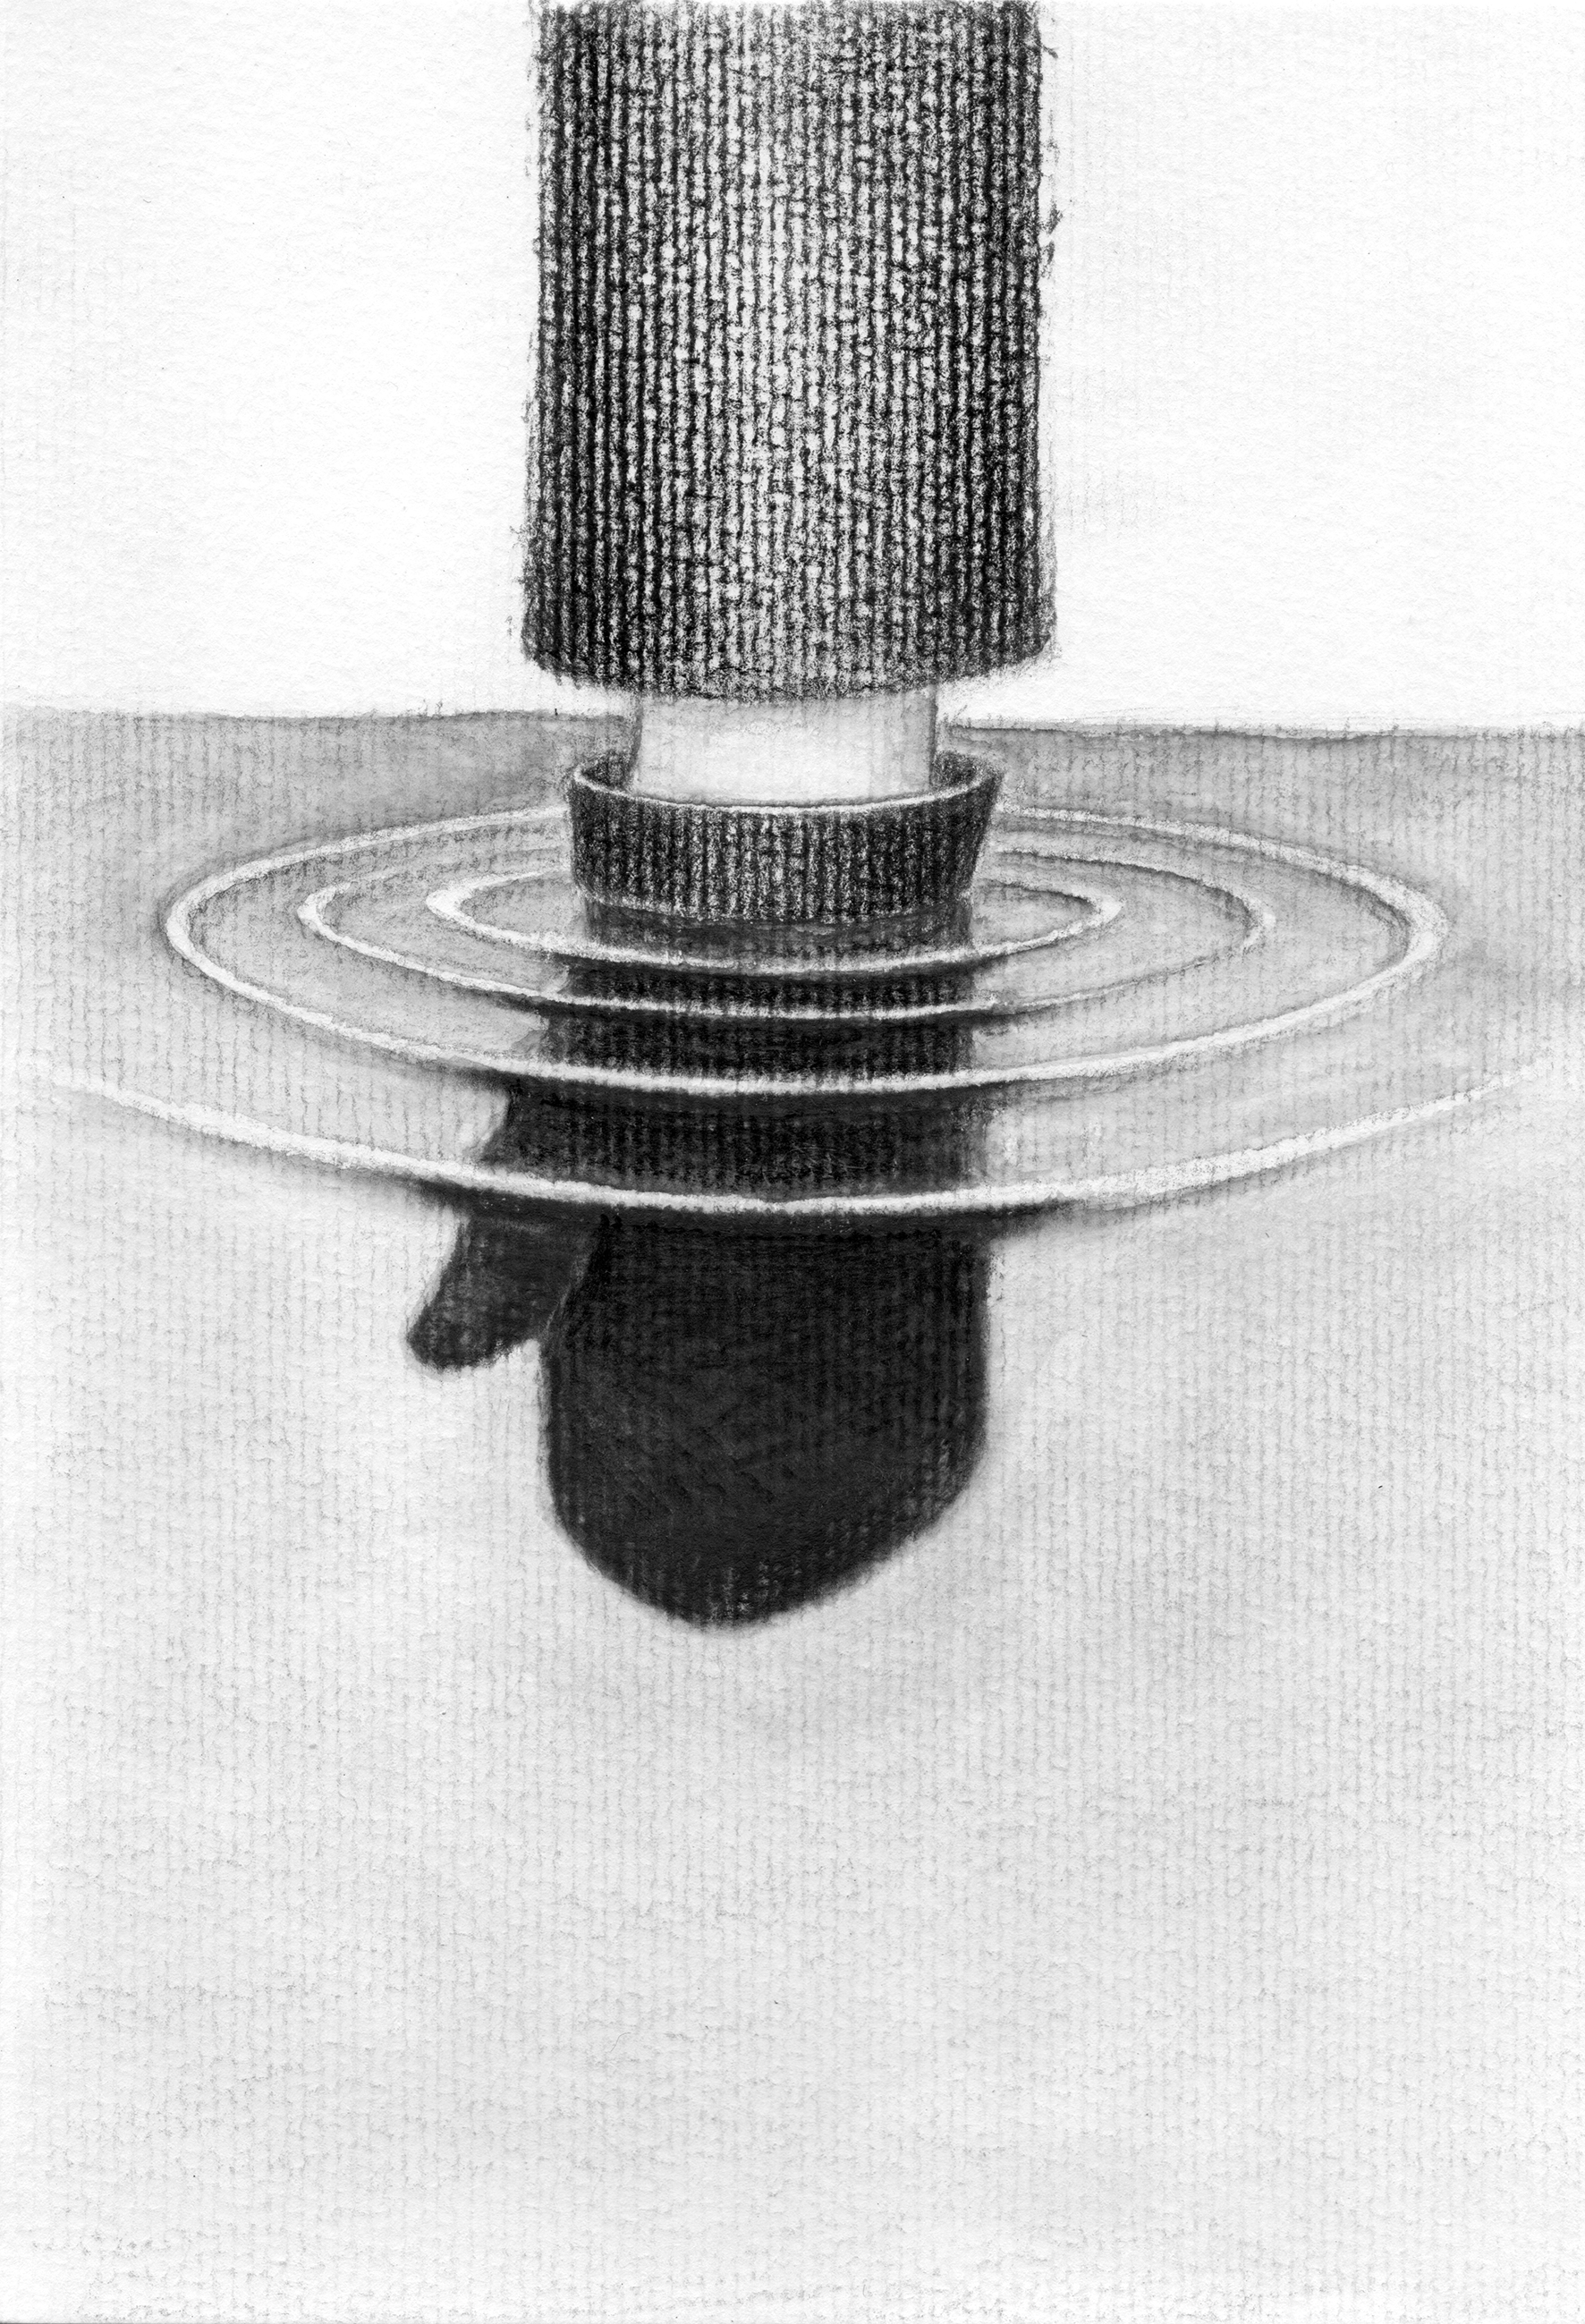
\includegraphics[width=8cm]{./img/4.pdf}
\legendas{Gravura de F. Valloton (\textit{Le cri de Paris}, 23 de janeiro de 1898, ilustrando a grande repercussão do caso.}
\end{figure}

Émile Zola nasceu em Paris em 1840, filho de mãe francesa e pai
italiano. Quando o menino tinha apenas sete anos, o pai morre e deixa a
família em condições difíceis. Mais tarde, o próprio Zola escreveria
que seus anos de infância e adolescência seriam cobertos de grande
miséria. Ainda assim, o futuro escritor se educa e aos 22
anos começa a trabalhar na livraria Hachette, onde permanece até os
26 anos. 

 A partir de então, Zola aproxima-se do jornalismo, colaborando com um
bom número de veículos. A proximidade com a imprensa, que se estenderia
por toda a sua vida --- inclusive depois que seus livros o tornam um
escritor consagrado --- possibilita-o viver de maneira modesta, mas com
condições razoáveis para se dedicar à ficção. 

Em 1871, Zola publica o primeiro volume do ciclo \textit{Os Rougon-Macquart}.
O livro alcança alguma repercussão, mas nada que se compare ao enorme
sucesso que, seis anos depois, \textit{A taberna}, o sétimo volume do
ciclo, alcançaria. 

Encerrada a coleção de volumes sobre os Rougon-Macquart, Zola
exercitaria sua inclinação pela série de romances com um segundo ciclo,
\textit{Trois Villes}, que seria composto por três volumes publicados entre
1894 e 1898. Mesmo depois do enorme desgaste que o caso Dreyfus lhe
traria, o escritor ainda tem fôlego para começar um outro ciclo de
romances, chamado por ele de \textit{Les Quatre Évangiles}. O primeiro volume,
publicado em 1899, viria a ter o sugestivo nome de \textit{Fécondité}.
Em 1901, sai o segundo romance, \textit{Travail}. O terceiro, de título
também muito significativo, \textit{Vérité}, é publicado em 1903, em
edição póstuma. O ciclo ficaria completo ainda com a publicação do
esboço, em estado avançado, do quarto volume, \textit{Justice}, no
mesmo ano.

 Financeiramente estável a partir do sucesso de \textit{A taberna}, o
escritor compra uma casa e estabelece uma vida familiar estável: sua
primeira filha, Denise, nasce em 1889. Dois anos depois Zola seria pai
de um menino, Jacques. A essa altura, o escritor já era considerado um
dos maiores do país e o sucesso de sua obra romanesca ultrapassara as
fronteiras da França. Além disso, os jornais recebiam suas colaborações
frequentes, que se estendiam do comentário literário à crônica
familiar, passando pela intervenção política. 

Zola publica o primeiro artigo sobre o caso Dreyfus em 1897. No começo
do ano seguinte, o jornal \textit{L'Aurore} estampa, na primeira página,
o famoso \textit{Eu acuso!} O texto toma conta de Paris e rende a Zola um
processo que o condenaria a um ano de prisão e uma multa de 3000
francos. No mês de julho, depois de ver a sentença confirmada por um
tribunal superior, o escritor foge para a Inglaterra para evitar a
prisão. De lá, continua sua atividade de escritor.

Depois de uma mobilização enorme, que movimentaria intelectuais de todo
o mundo, em junho de 1899 o processo do capitão Dreyfus começa a ser
revisto. Com a notícia, depois de 11 meses no exílio voluntário, Zola
retorna à França. Um mês depois, aliás, o próprio Dreyfus desembarcaria
em solo francês. O país continua abalado pelo caso, o que faz com que
o escritor permaneça no centro dos debates. No final de 1900, uma lei
anistia todos os envolvidos.

A participação de Zola no caso nunca foi completamente aceita pela
sociedade francesa. Enquanto uns o aplaudiram pela bravura e dignidade,
separando-lhe a alcunha de “intelectual verdadeiro”, outros o
tratavam --- como a todos os que ousaram defender Dreyfus já no calor dos
acontecimentos --- como um traidor.

Em 1902, Zola é encontrado morto em circunstâncias misteriosas: com a
saída da chaminé obstruída por algumas pedras, ele se asfixia. Ainda
hoje, suspeita-se de que o grande escritor foi vítima de assassinato.
\asterisc

\begin{figure}
\centering
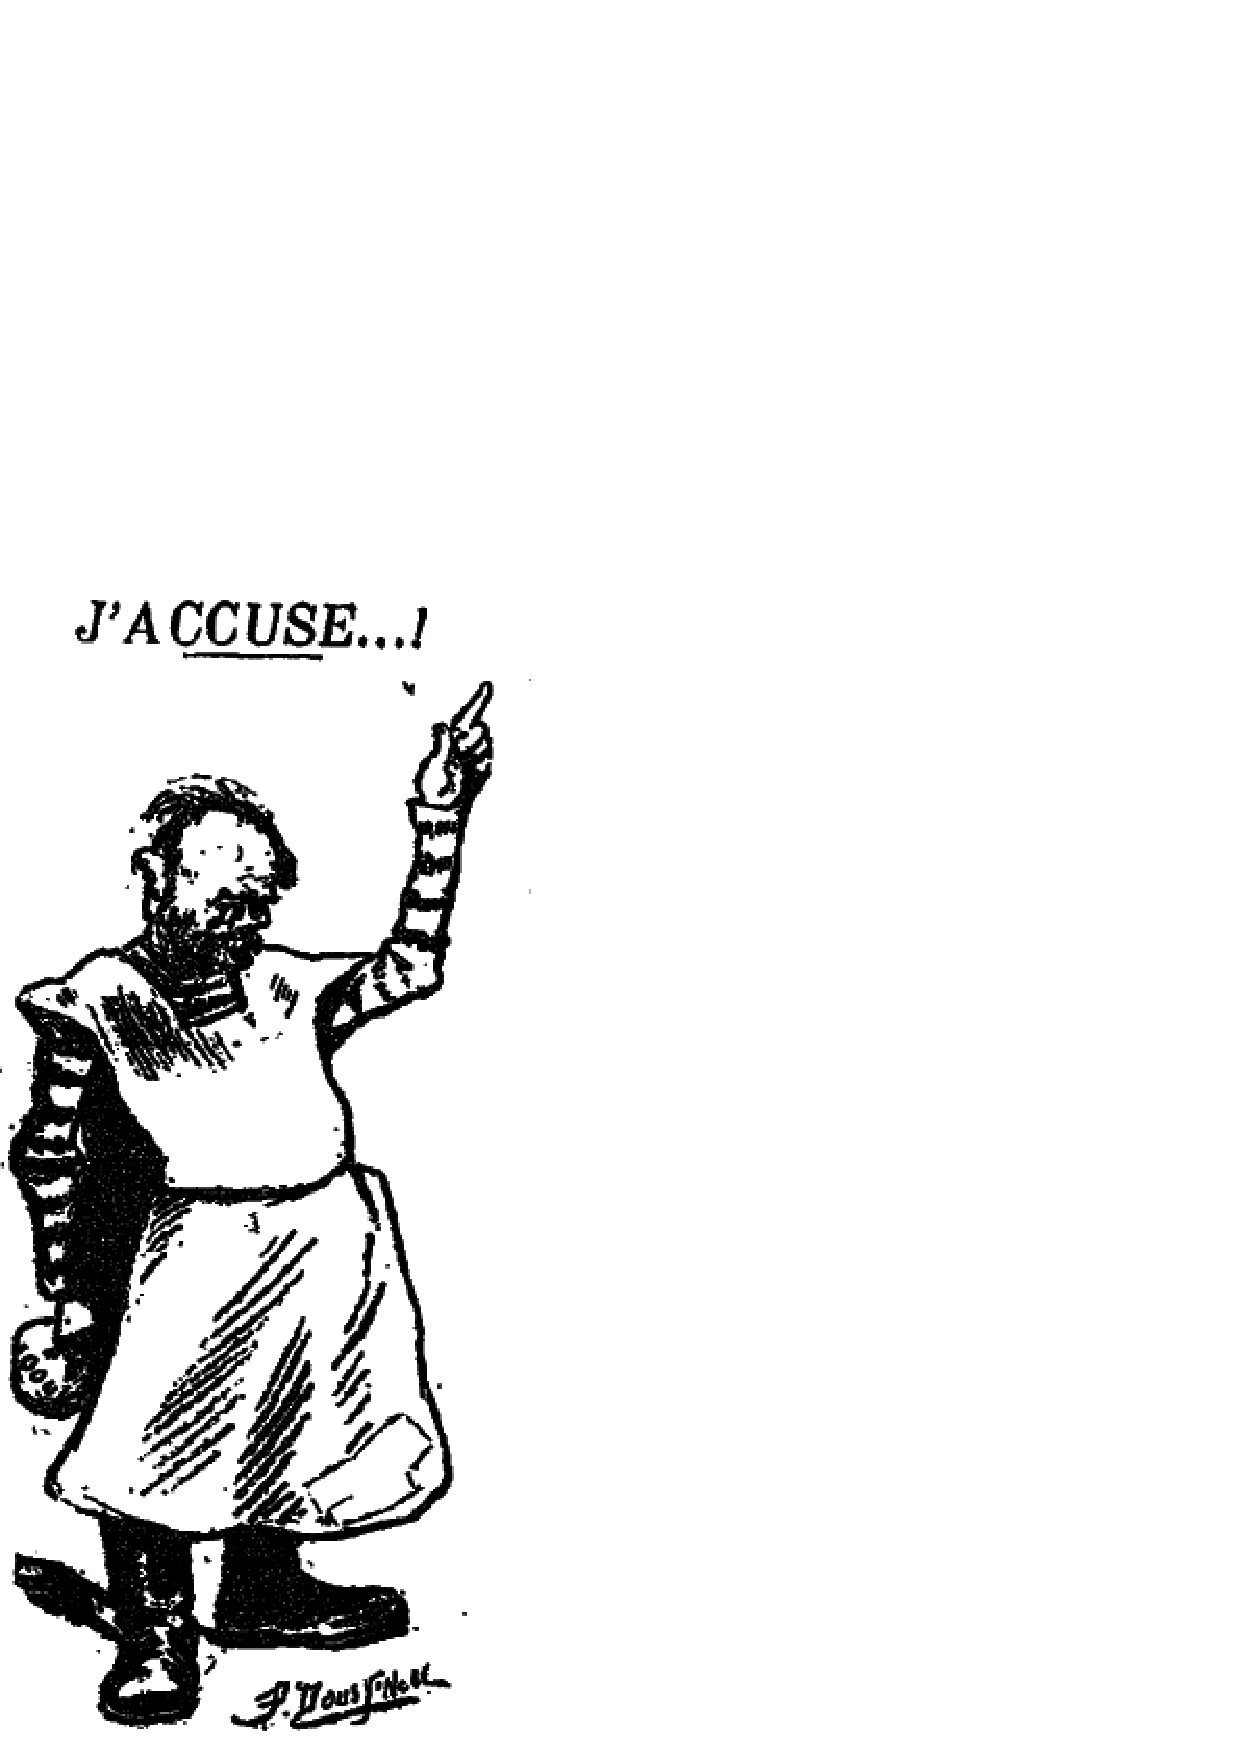
\includegraphics[width=5cm]{./img/43.pdf}
\ \\
\legendas{Caricatura de Zola publicada no jornal \textit{La Patrie} no artigo de Emile Massard \textit{Je prouve\ldots! Pas de Phrases, des Faits!} [Eu aprovo\ldots! Nada de frases, aos fatos!]}
\end{figure}

O chamado caso Dreyfus é um dos mais conhecidos erros
judiciais da era moderna. A partir da interceptação de uma carta, em
setembro de 1894, cujo conteúdo teria segredos estratégicos, o Estado"-Maior
francês sai à busca de um culpado e depois de breves investigações
chega ao capitão Alfred Dreyfus, acusado aparentemente segundo algumas
evidências grafológicas, elas mesmas, aliás, duvidosas.

 A acusação de traição torna-se ruidosa e a França se vê ansiosa por
achar um culpado. O judeu Dreyfus, em uma sociedade em que o
anti-semitismo começava a crescer (e culminaria no vergonhoso apoio
às políticas racistas da Alemanha de Hitler), torna-se um suspeito
facilmente condenado pela opinião pública e, no final daquele mesmo ano,
um conselho de guerra o obriga ao degredo na ilha do Diabo, além de
expulsá-lo do Exército, com um ato de humilhação pública. 

 O julgamento é vergonhoso e chama atenção de intelectuais de todo o
mundo: como as provas eram, sem nenhuma razão, secretas, o advogado de
Dreyfus nem sequer sabia do que exatamente deveria defender seu cliente.
Apenas os juízes tiveram acesso a um “documento” que traria provas
irrefutáveis contra o capitão. No início de 1895, com a punição sumária
engasgada para uma parte da intelectualidade francesa --- e, como se verá no
caso de Rui Barbosa, do resto do mundo ---, Dreyfus é enviado para o
degredo. Grande parte da população se vê aliviada, mas para alguns a
pena seria desproporcional. As irregularidades do processo, porém, não
permitiriam que o assunto deixasse os jornais e, aos poucos, nomes
ilustres começam a aparecer entre os “dreyfusards”, como ficaram
conhecidos aqueles que se dedicaram à defesa do capitão: além de Zola,
Anatole France e Marcel Proust figuram entre os escritores que
assinaram manifestos, escreveram artigos ou, com mais força, fizeram da
causa de Dreyfus uma espécie de ideal ético.

O caso começa a ter uma reviravolta quando, em 1896, o tenente"-coronel Picquart, 
que assume um posto estratégico dentro do Exército, diz que
possui evidências muito fortes de que, na verdade, o autor da carta que
culminou com o degredo de Dreyfus era o comandante Esterhazy. Com uma
manobra rápida, o Exército isola Picquart e o transfere a uma
localidade distante da França. Àquela altura, porém, o caso já tinha
tomado enormes proporções: em 1897 o irmão de Dreyfus, Mathieu, vai aos
jornais e acusa Esterhazy de ser o verdadeiro culpado. 

 É aqui que Zola resolve se engajar firmemente no caso e começa a
redigir uma série de artigos. O primeiro sairia no \textit{Figaro}, em
25 de novembro de 1897. Não conseguindo apoio imediato dos jornais,
Zola lança um folheto independente ainda no final daquele ano. O texto
é dirigido à juventude e já apresenta momentos da exaltação apaixonada
que dominaria os artigos do ano seguinte. No início de 1898, sai outra
brochura, com Zola agora se dirigindo à França e apelando para o
retorno à dignidade de um país que teria um histórico de lutas pela
justiça.

 O jornal \textit{L'Aurore}, então, que já havia tomado a defesa de
Dreyfus, acolhe o artigo mais importante de toda a série:
\textit{Eu acuso!}, que, sob a forma de uma carta aberta ao presidente
Félix Faure, balança todo o país. Já bastante familiarizado com o caso,
Zola logo de início apresenta o nome dos envolvidos e depois descreve o
Conselho de Guerra que havia condenado Dreyfus, demonstrando como o
processo inteiro foi tomado por impropriedades, pressa e, no limite,
desonestidade. Zola, sempre bastante exaltado, como a ocasião convinha,
revela a patética figura do comandante Esterhazy, que já havia sido
denunciado, aliás, pelo irmão de Dreyfus, e, depois, chama atenção para
o fato de que a corte se contaminara pela comoção que assolou o país e
boa parte da imprensa.

 O texto chega ao auge nos últimos parágrafos quando Zola enfileira a
culpa de cada um dos envolvidos, iniciando oito frases com o verbo
“acuso”, que, dessa maneira, ecoa fortemente no leitor. O final é
surpreendente: o escritor adianta que conhece os artigos da lei a que
pode ser acusado por ter redigido aquele tipo de texto. Na conclusão,
Zola admite que sua estratégia é justamente fazer o tema voltar à
justiça para, então, poder apresentar diante da corte as provas que lhe
pareciam incontornáveis.

 De fato, poucos dias depois da publicação de \textit{Eu acuso!}, o ministro
da Guerra entra com uma queixa e a justiça intima Zola. O escritor,
então, publica novo texto: aqui, faz um juramento pela inocência de
Dreyfus, colocando inclusive sua própria obra como garantia. O barulho
que os textos de Zola causam não parece impressionar os juízes, e a
Corte o condena à multa e prisão, o que acabaria por levá"-lo ao
exílio. 

Uma chuva de protestos, vinda de todos os lados, toma conta da França. A
solução a que o caso chega termina sendo política, e não judicial: o
presidente --- depois de uma revisão --- resolve “perdoar” Dreyfus e
anistiar todos os envolvidos no caso, depois que o processo passa por
uma revisão e a culpa de Dreyfus é “atenuada”. Zola encerra o exílio,
mas não sua intervenção: mais alguns textos são publicados no
\textit{L'Aurore}: em alguns, o escritor analisa a decisão da anistia,
reafirmando sua convicção pela inocência de Dreyfus e, inclusive,
dizendo que, diante da gravidade dos acontecimentos, \textit{Eu acuso!} era
um texto comedido; em outros, dirige-se à própria esposa do capitão,
que voltava do degredo, para consolá-la.

Em 1901, com os acontecimentos ainda em curso, Zola reúne todos os
textos que havia publicado sobre o tema em um livro que, se não fosse a
terrível veracidade do conteúdo, talvez pudesse ser considerado um de
seus melhores romances. Aliás, é um bom exercício lê-lo a partir de
alguns pressupostos romanescos: juntos, os artigos compõem um painel
razoavelmente fragmentário, em que as personagens são compostas segundo
a ordem de culpa e degradação em um fato que é, desde o início, dado
como de amplo conhecimento do leitor. 

Quatro anos depois da morte de Zola, o Exército francês finalmente
admite o erro e reintegra Alfred Dreyfus, que chega a receber uma
medalha da Legião de Honra. O caso, porém, não arrefeceria: em 1908,
enquanto participava da cerimônia de transferência das cinzas de Zola
ao Panthéon, Dreyfus leva dois tiros no braço, desferidos por um nacionalista exaltado, 
o jornalista Gregori. Dreyfus morreu em 1935, sem nunca ter deixado, de um jeito ou de
outro, de sair dos jornais e do debate político francês e internacional.
\asterisc

\begin{figure}
\centering
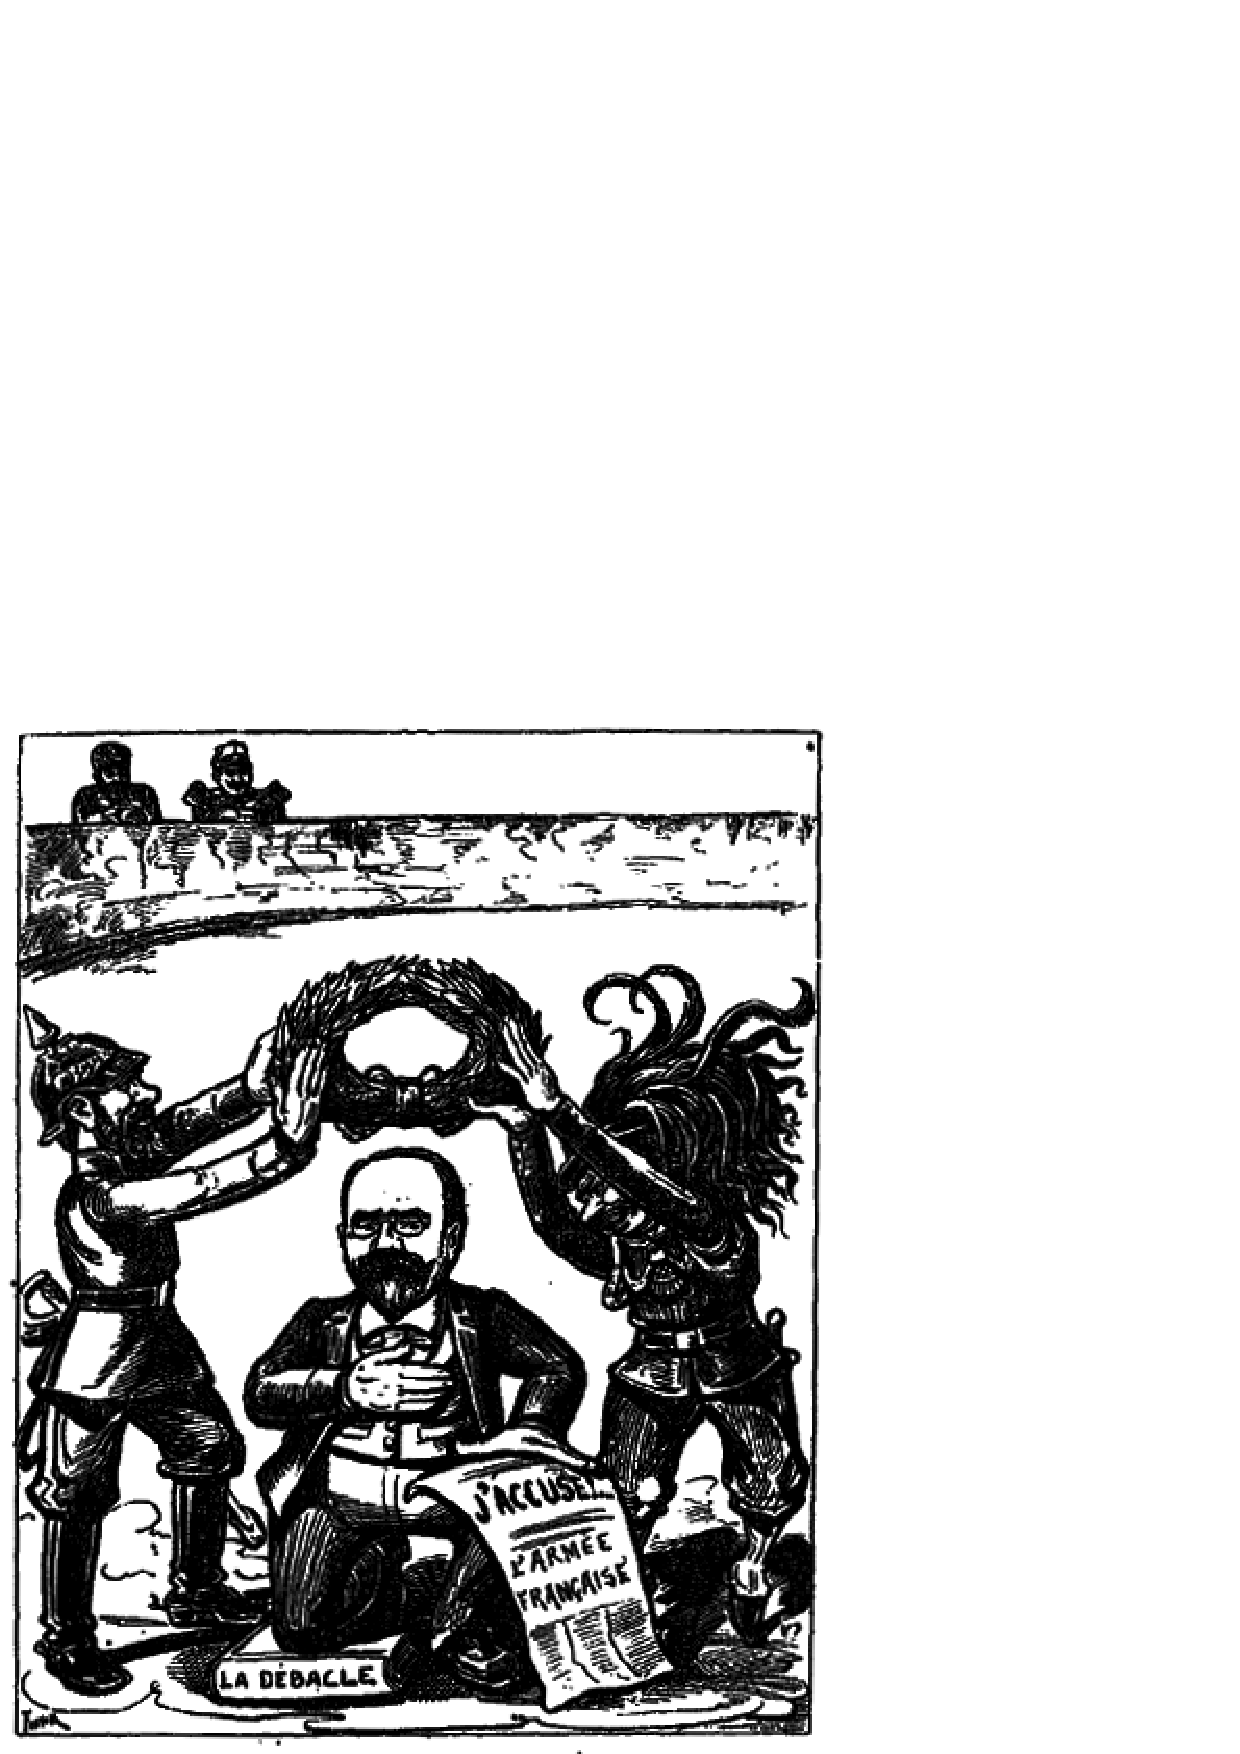
\includegraphics[width=8cm]{./img/131.pdf}
\legendas{Ilustração de Par Fertom (\textit{Le Pilori}, 23 de janeiro de 1808). 
``Coroamento de uma carreira'', ``\textsc{zola} --- `Obrigado, camaradas, 
vocês ao menos me fizeram justiça'. ''}
\end{figure}


O caso Dreyfus, de maneira geral, e, mais particularmente, o
\textit{Eu acuso!}, de Émile Zola, tiveram uma enorme repercussão no
pensamento filosófico e jurídico da época e também das décadas
seguintes. Um dos estudos mais agudos é o capítulo dedicado ao assunto
que Hannah Arendt publicou em \textit{O sistema totalitário}.\footnote{Hannah 
Arendt, \textit{O sistema totalitário}, Lisboa, Dom Quixote, 1978, p.
179. A frase, no livro, aparece invertida: “Assim termina o único
episódio no qual as forças subterrâneas do século \textsc{xix} vêm à plena luz
nos registros da história.”}  O texto da filósofa tem a vantagem de 
observar as consequências do caso de uma
maneira ampla, inclusive para o desenvolvimento do pensamento
nacionalista europeu, que culminaria, entre outros desenvolvimentos,
no nazismo alemão. Além disso, Arendt tem o mérito de contextualizar o
caso na política francesa, demonstrando como parte da defesa que se
formou em torno de Dreyfus tinha interesses que iam além da mera
justiça.  No entanto, o texto reduz a participação de Émile Zola a uma
espécie de mero arrazoado apaixonado, que às vezes ela chega a
classificar de patético, sem contextualizá-la nem com a obra do autor
de \textit{Germinal} e muito menos compreender seus textos a partir do
estilo que, no caso, exigiria que Zola, de fato, lançasse altas doses de
emoção, já que pretendia --- como Arendt, aliás, nota --- transformar
inclusive a opinião pública, àquela altura manipulada por parte da
imprensa e, em sua maioria, contra o capitão Dreyfus. 

Ainda que não observe aspectos da forma literária, o maior ganho do
texto de Arendt é a instalação do caso Dreyfus num contexto histórico
que teria a curiosa característica de, em suas palavras, expor “à plena
luz as forças subterrâneas do século \textsc{xix}”. Curiosamente, 
e a observação é da própria Arendt, o caso expõe ainda alguns dos traços 
históricos do século \textsc{xx}, um deles o anti-semitismo.\footnote{ De passagem, ainda, vale repetir
que literariamente Émile Zola também instaurou \textit{Eu acuso!} dentro
das novas manifestações artísticas que surgiam com a modernidade que,
segundo Malcolm Bradbury, “gerou algumas das obras literárias mais
geniais e perturbadoras que conhecemos, e algumas das mais dolorosas
\textit{manifestações da autoconsciência} e da ansiedade modernas”. (Grifo nosso.)  }

Para a autora de \textit{Eichmann em Jerusalém}, o fato de Dreyfus ser
judeu foi decisivo em sua condenação e, depois, na oposição que a
opinião pública lhe dedicou. O fato é indiscutível. Como o assunto
tomou proporções internacionais, com protestos vindos de todos os
cantos do mundo, o caso Dreyfus teria tido como “único resultado
visível o nascimento do movimento sionista --- a única resposta política
que os judeus encontraram para o anti-semitismo, e a única ideologia
a qual chegaram a levar a sério o comportamento hostil, que os
impeliria para o centro dos acontecimentos mundias”.\footnote{ \textit{Idem, ibidem.}} 
Se pensarmos nos conflitos do Oriente Médio e na política
preventiva contra o povo palestino, por exemplo (ou para ir mais
longe, em todo tipo de guerra preventiva que toma conta do mundo
contemporâneo), de imediato fica claro o alcance do “erro judiciário”
cometido contra o capitão Alfred Dreyfus no ano de 1894.\footnote{ Como
detalhe auxiliar, que talvez interesse mais aos psicanalistas que aos
filósofos, Arendt lembra ainda que o caso Dreyfus não teve um desfecho
jurídico, ficando em aberto com a anistia geral (sublinha ela que
ilegal) concedida a todos os envolvidos no caso. Simbolicamente --- e
agora a observação é minha ---, um desfecho no âmbito legal talvez tivesse
sido útil para minorar as graves consequências do caso.} 
\asterisc

Interessante para nós brasileiros, e para aqueles que se interessam
pelo caso no plano jurídico, é um texto que Rui Barbosa redigiu, logo
depois dos primeiros julgamentos e da condenação, no começo de 1895, e
enviou, da Inglaterra, para o \textit{Jornal do Commercio}, no Rio de
Janeiro. O texto de Rui Barbosa é baseado em notícias da imprensa e em sua
intuição de jurista e alinhava questões políticas a princípios
jurídicos para expor a ilegalidade e a inconsistência do processo. Não
existe sinais da repercussão do texto na Europa (muito menos na
França), mas por aqui o estudo de Rui Barbosa circulou e chegou a ser
publicado em Buenos Aires.

\begin{figure}
\centering
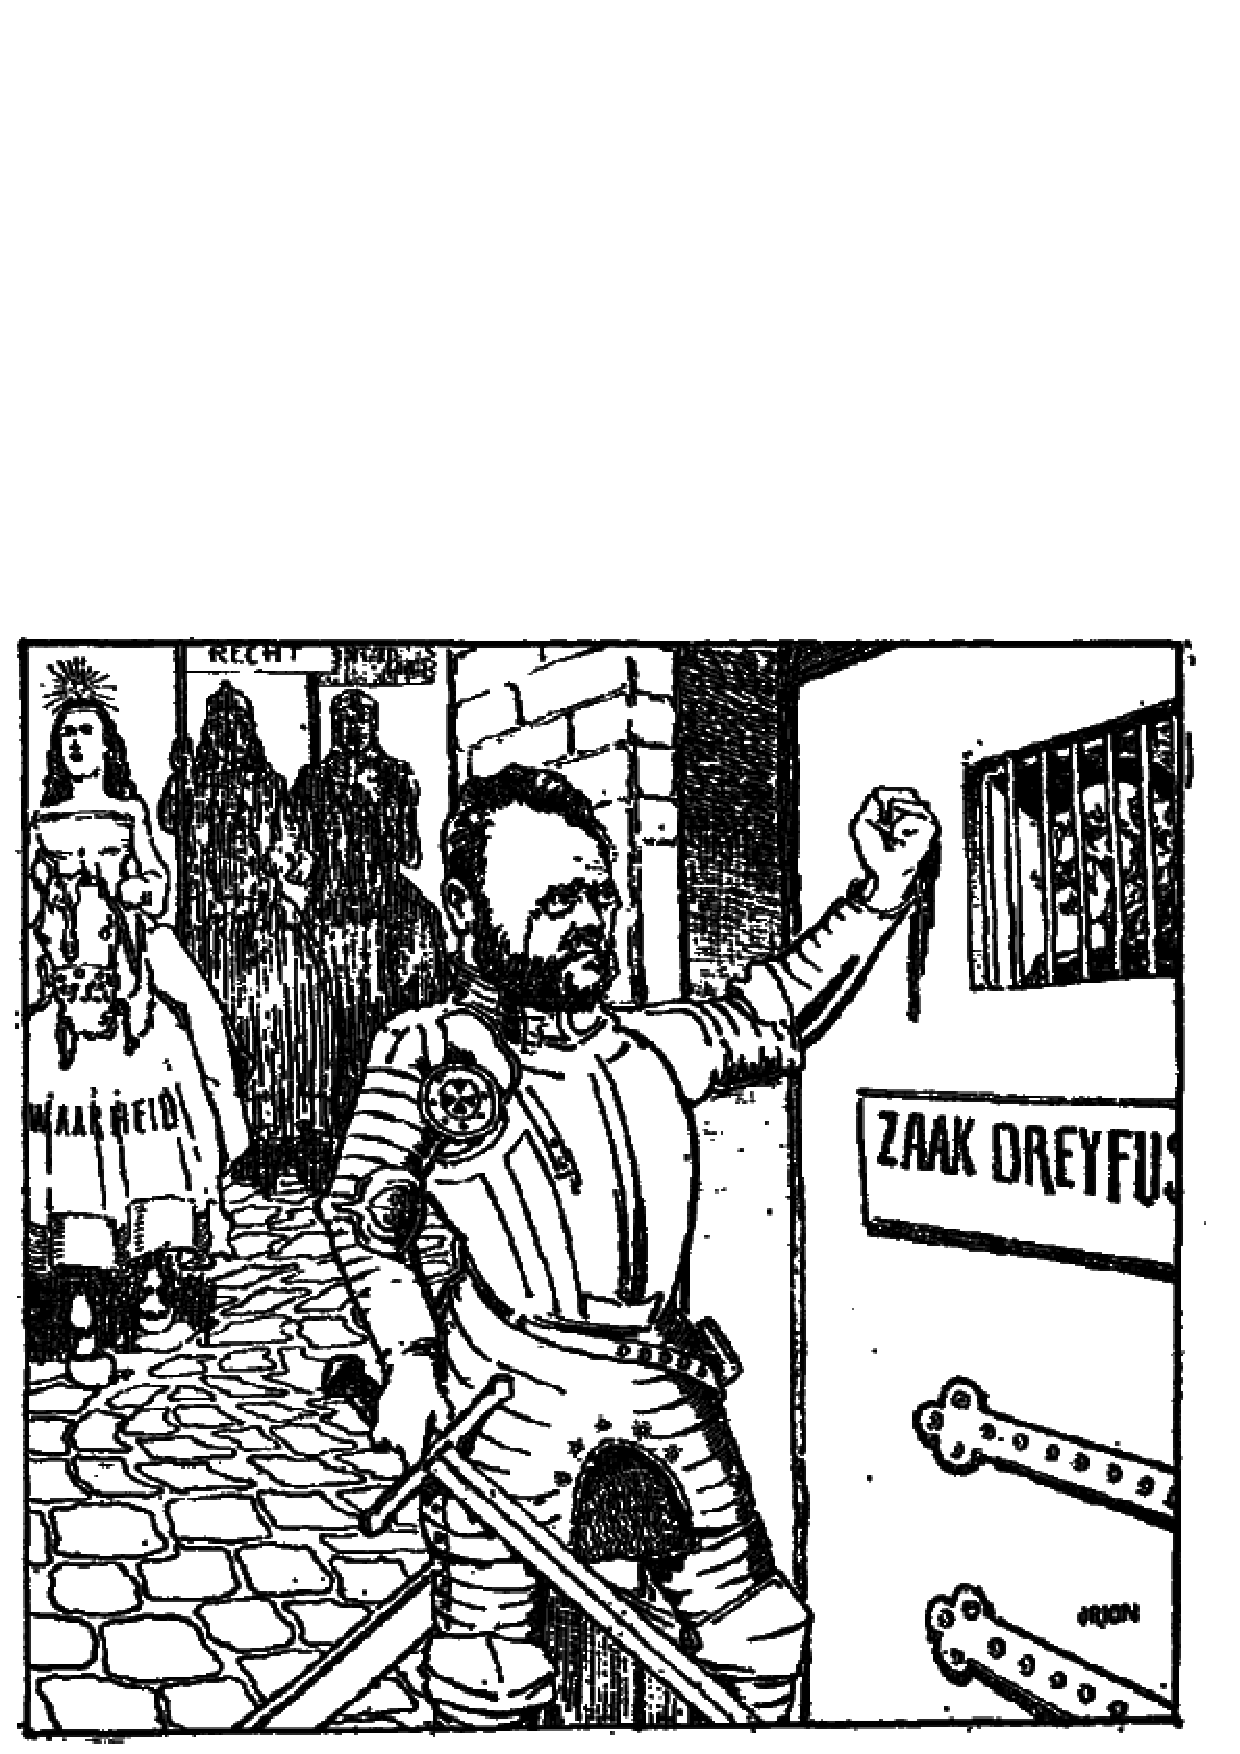
\includegraphics[width=8cm]{./img/250.pdf}
\legendas{``\textsc{zola} --- Abra! A verdade, o direito e a liberdade exigem!\\
\textsc{um general} (de dentro da sala)  --- Não entrarão!\\
\textsc{zola} Não? Então, violência. Eu forcarei a porta com a\\minha espada.''\\
(\textit{Nederlandsche Werkman}, Holanda, 5 de fevereiro de 1898)}
\end{figure}

 O cerne do texto de Rui é uma comparação entre o sistema judicial
francês e o inglês: segundo ele, esse último jamais permitiria ser
influenciado pela opinião pública, decisiva no caso Dreyfus.
Obviamente, o jurista brasileiro pende para o lado da “frieza”
britânica, chegando mesmo a insinuar se não haveria algo de “latino” na
propensão de alguns povos por condenar antes de qualquer julgamento. No
caso de Dreyfus, inclusive antes de qualquer julgamento e sem nenhuma
prova concreta.

 Rui Barbosa aponta ainda a inconsistência absoluta da única prova
que existiria contra Dreyfus, o famoso “documento”, que permaneceu o
tempo inteiro secreto, e cuja autenticidade não se pode contestar, já
que quando o advogado do acusado tentou fazê"-lo teve a voz cortada.
O tom do artigo é frio e grande parte dele é coberta por uma espécie de
resumo da imprensa inglesa sobre o caso. Além disso, o texto de Rui Barbosa se
diferencia do de Zola pela recusa a qualquer emotividade --- lembrando,
outra vez, que o jurista brasileiro focava outro público.

 No entanto, há uma coincidência curiosa e interessante: tanto Rui
quanto, depois, Zola chamam atenção para a falta de motivações
concretas para um homem como Alfred Dreyfus cometer um crime como
aquele. Nessa altura, o trecho de Rui Barbosa parece, depois, ter ecoado na
pena de Zola: 

\begin{hedraquote}
Ora, Dreyfus não tinha no seu passado uma nódoa, um
traço duvidoso. Quinze anos de serviços imaculados e a alta posição de
confiança, que ocupava no mais delicado ramo da administração da
guerra, definem-lhe a fé de ofício. A superabundância de seus
recursos, a opulência de sua família, a simplicidade de seus hábitos,
a sua aversão ao jogo, a concentração exclusiva de sua vida particular
nas afeições domésticas excluem a suspeita das seduções tenebrosas, que
são frequentemente a explicação obscura dessas catástrofes da honra.
\end{hedraquote}

Se acrescentarmos a tinta da indignação e um estilo mais veemente,
podemos encontrar eco do trecho citado em diversas passagens de Zola,
como quando ele lista algumas das qualidades de Dreyfus: 

\begin{hedraquote}
Dreyfus domina vários idiomas: crime; não há um papel sequer em
sua casa que o comprometa: crime; de vez em quando ele retorna à sua
pátria: crime; trabalha muito, tem o cuidado de se informar sobre tudo:
crime; não perde a calma: crime; perde a calma: crime.
\end{hedraquote}

Obviamente, não há nenhuma importância na vantagem cronológica do texto
de Rui Barbosa. A comparação com o de Zola, no entanto, é lucrativa se
observarmos questões de estilo: o brasileiro, ainda que sem fazer uso
de termos técnicos, procurava alinhavar argumentos jurídicos, colocando
lado a lado duas jurisdições para concluir pela vantagem da
independência britânica quanto ao clamor popular. Além disso, Rui
aponta a inconsistência da necessidade do segredo e, ao mesmo tempo, do
ocultamento da única prova contra Dreyfus, já que o assunto poderia ser
tratado por ambas as partes no interior do tribunal.

Zola, por sua vez, e até porque escrevia três anos depois, quando os
acontecimentos tinham tomado proporções gigantescas, não se preocupa
com alegações jurídicas, já que para ele a questão estava mais do que
estabelecida. Para o grande escritor, a verdade está exposta e precisa
apenas chegar aos donos do poder, que estariam manipulando interesses
subterrâneos, para adotar a linguagem de Hannah Arendt, e ao mesmo
tempo sendo manipulados pela opinião pública, desde sempre irracional,
como o próprio Rui Barbosa faz questão de lembrar.

A diferença entre os dois textos, portanto, é de estilo: cada um dos
autores precisa adequar suas ferramentas de redação para redigir algo
coerente e que obtivesse o efeito desejado. Rui Barbosa, sem sombra de
dúvidas e assumidamente, objetivava expor para o Brasil o bom
exemplo da justiça britânica e, ao mesmo tempo, demonstrar o perigo
para a justiça quando as emoções falam mais alto. Zola, por sua vez,
precisava enfrentar essa emoção a ponto de fazer o público observar
verdades que para ele, àquela altura, já eram inquestionáveis. Já que
estamos falando de ferramentas formais, adequação de estilo e termos de
linguagem, temos toda a tranquilidade para concluir que os textos de Rui
Barbosa e de Émile Zola, sobretudo o desse último, estão no âmbito da
literatura. 
\asterisc

\begin{figure}
\centering
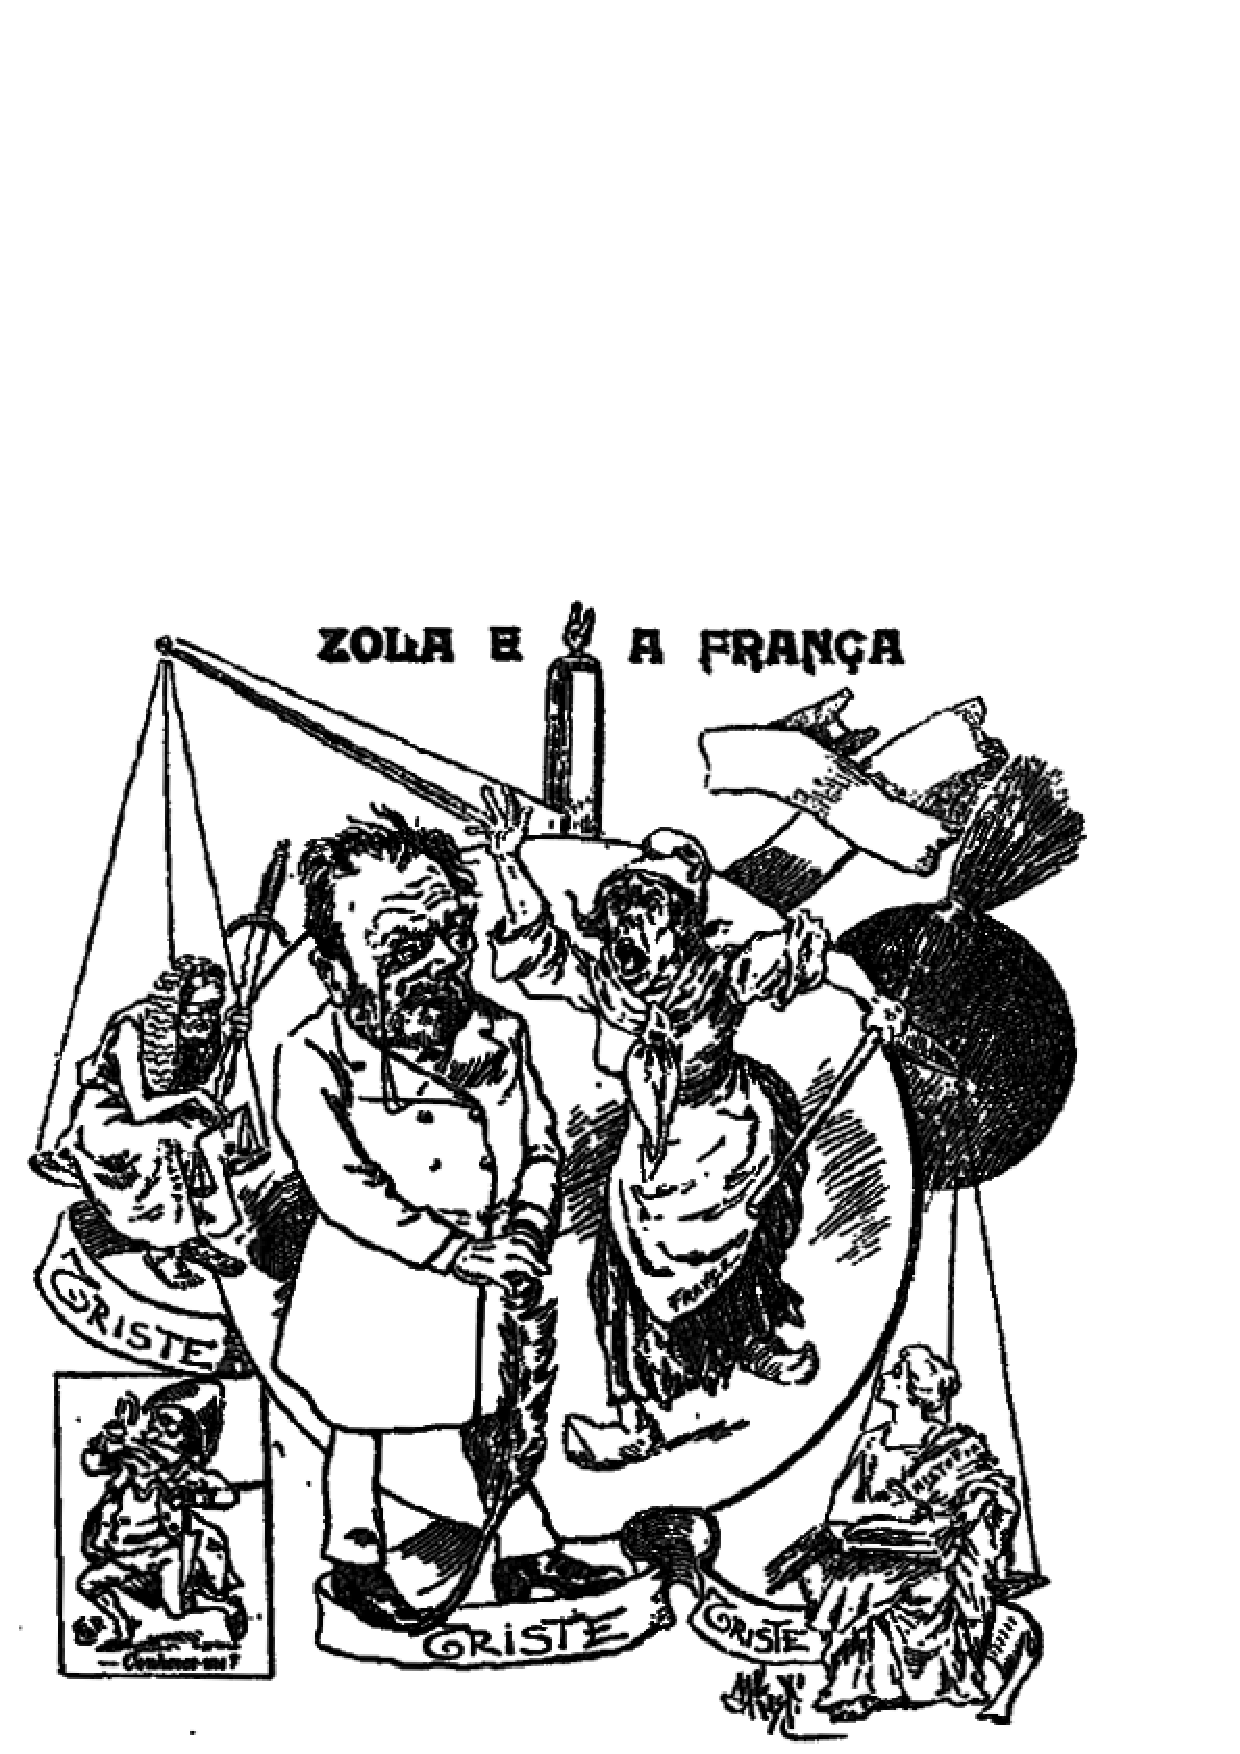
\includegraphics[width=8cm]{./img/279.pdf}
\legendas{Caricatura de R. Rordallo Pinheiro, para o jornal de Lisboa \textit{Antonia Maria} (17 de fevereiro de 1898).}
\end{figure}

Com o passar dos anos, enquanto o século \textsc{xx} mergulhava na escuridão
bélica que o abateria algumas vezes, o texto de Zola foi se tornando
menos valorizado até que, em algum momento, começou a ser chamado de
“panfleto”: algo que, por ter um teor de propaganda política explícita,
não alcançaria nenhum valor estético. A propósito, valeria a pena
investigar os diversos sentidos que a palavra “panfleto” carregou --- aos
moldes do clássico vocabulário de Raymond Williams\footnote{
Raymond Williams, \textit{Palavras-chave}, São Paulo, Boitempo,
2007.} --- para descobrir quando exatamente o termo tornou-se
pejorativo. Nesse momento, a teoria literária (e também o discurso que
os artistas procuram formar sobre seu próprio trabalho) viu-se em
meio a uma enorme confusão.

Entre tantos, um dos paradoxos intelectuais do século \textsc{xx} é o que
contrapõe esse fato, a produção de um discurso que procura esvaziar a
arte de qualquer sentido político, ao desenvolvimento da linguística,
que aponta justamente para a existência de um ato político por trás de
toda manifestação de linguagem. No Brasil contemporâneo, inúmeros
setores ligados à literatura repetem à exaustão o clichê: literatura e
política são dois planos separados. 

Uma das consequências nefastas do discurso de separação entre estética
e política é a desqualificação da figura do escritor como um produtor
de intervenção no seu próprio tempo. Obviamente, não defendo a
superioridade da opinião do artista sobre qualquer outra, mas é fácil
ver que, tal foi a diluição da forma literária no vazio ideológico, o
escritor tornou-se irrelevante no que toca à emissão de qualquer
discurso que não seja o imediatamente associado à sua assim chamada
“obra”, ficcional ou de qualquer outro gênero.
\asterisc

 Entre tantas particularidades, a tradução de \textit{Eu acuso!} procurou
manter em língua portuguesa a veemência do texto de Émile Zola. As
diversas frases exclamativas foram vertidas para o português, o tom 
indignado foi mantido, e a sintaxe direta, conservada. Fizemos pequenas
alterações de pontuação apenas onde o sentido exigia. 

Apenas um termo merece destaque, justamente o mais importante de todo o
texto: o tal \textit{bordereau}, que seria a origem de todo o caso Dreyfus. O
suposto documento que continha informações confidenciais sobre a segurança
francesa, encontrado com os alemães e atribuída a Dreyfus, é
apresentado por Zola como \textit{bordereau}. Como sublinhamos, nem a defesa
do acusado pôde ter acesso a esse “documento”. Enquanto o texto se
desenvolve, \textit{bordereau} acaba significando as provas que a justiça
oculta e, ao mesmo tempo, usa para condenar os acusados de traição.
Dessa forma, optamos por utilizar o cartorial “documento”, para
traduzir, \textit{bordereau}, mantendo assim o caráter de papel desconhecido
que Zola tentou imprimir ao termo, ao mesmo tempo que dava certo ar de
patético à solene ilegalidade do processo. 

\begin{figure}
\centering
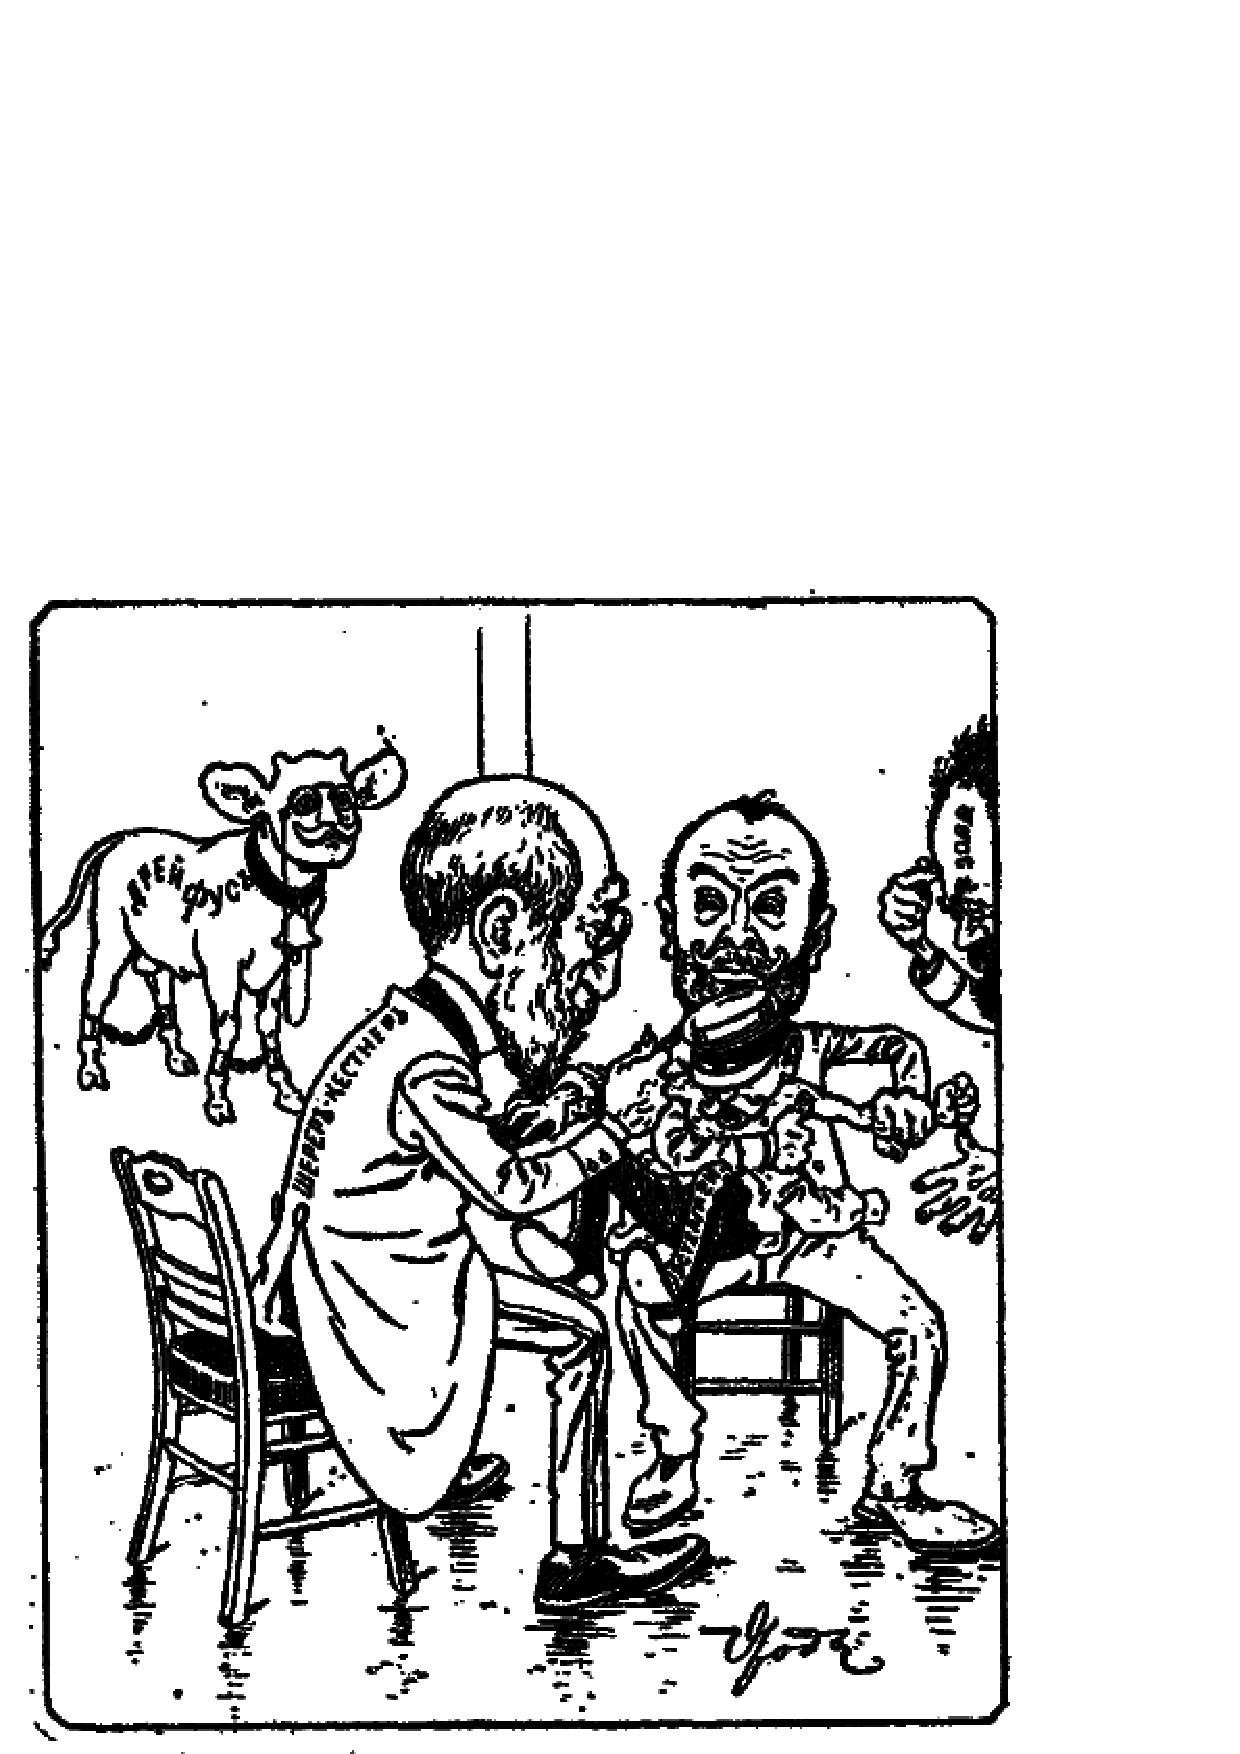
\includegraphics[width=8cm]{./img/284.pdf}
\legendas{Scheurer"-Kestner, diante de Zola, aplica uma vacina de traição no major
Esterhazy, produzida com o sangue do novilho Dreyfus.
(\textit{Strekoza}, São Petersburgo, Rússia, janeiro de 1898).}
\end{figure}

 A presente tradução foi baseada na edição da Librio, publicada em
francês com apresentação de Philippe Oriol em 1998. Aqui e ali observamos
as soluções encontradas pela tradutora da edição inglesa, Eleanor
Levieux, publicada pela editora da Universidade de Yale, em 1996. Por
fim, consultamos também a tradução brasileira, publicada pela extinta
Edições Atlanta, no Rio de Janeiro. 

